\chapter{Fundamentação Teórica}
\label{chap:fund}

Neste capítulo serão apresentados os principais tópicos relacionados ao <Assunto Estudado>, seu conceito e seus impactos na sociedade, bem como as motivações para suas publicações e formas de identificá-las. Além disso, serão abordadas técnicas que permitem <Descrever as técnicas utilizadas>, que serão aplicados para <Tema Proposto>. 

\section{Conceito 1}
\label{sec:conceito1}

Abaixo é apresentada uma figura com o logotipo do Instituto Federal de Santa Catarina. Para inserir uma figura usando o LaTeX, utilizamos a diretiva \emph{figure}. Normalmente referenciamos a figura a partir do seu label, conforme segue. A Figura \ref{fig:exemplo1} mostra o exemplo de uso de imagenos no \LaTeX.

\begin{figure}[!htb]
    \centering
    \caption{Exemplo de uso de imagens no \LaTeX.}
    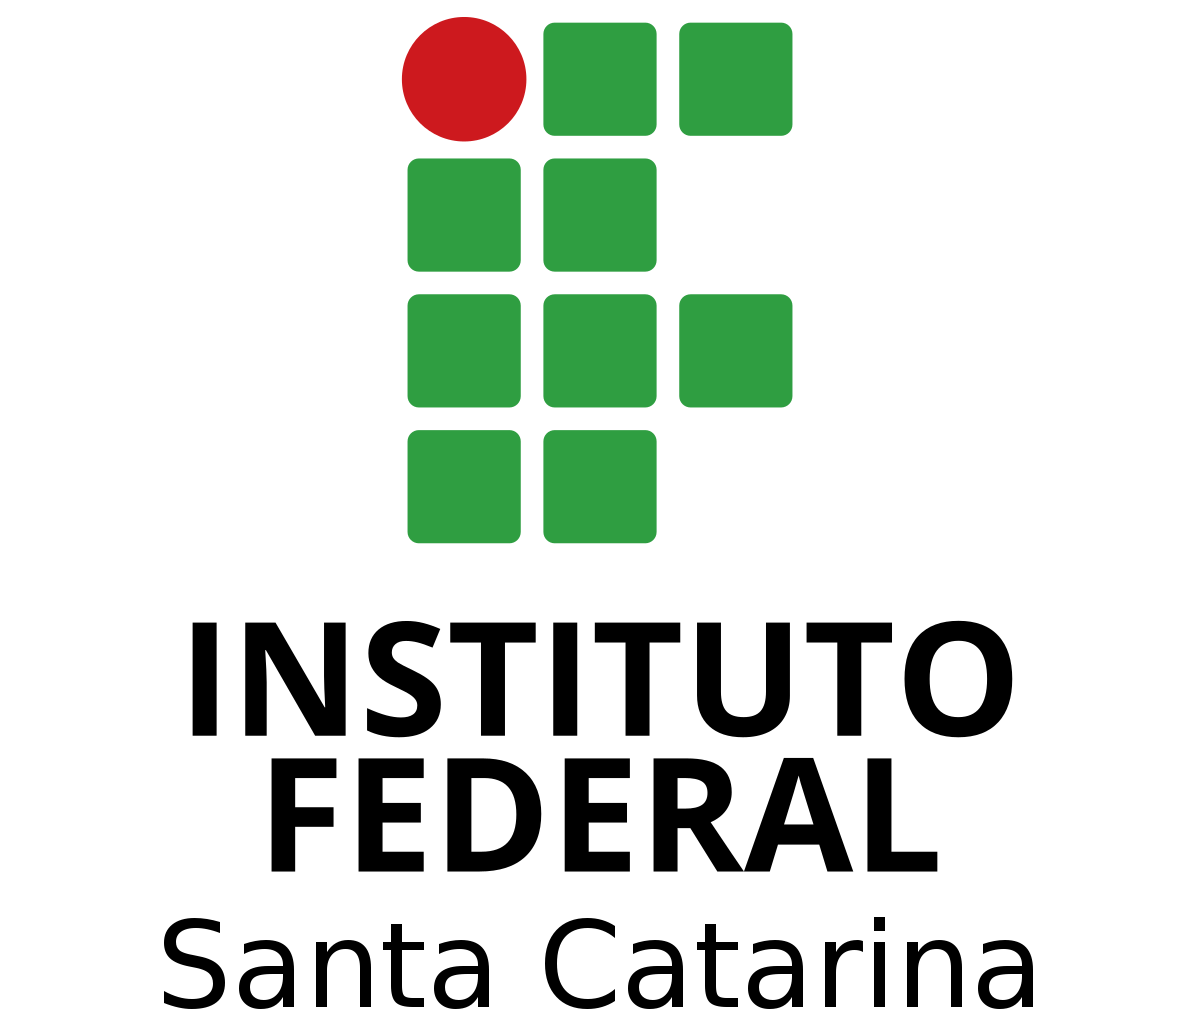
\includegraphics[width=0.40\textwidth]{img/ifsc.png}
    \legend{Fonte: Elaborada pelo autor.}
    \label{fig:exemplo1}
 \end{figure}
 
 Observe todos os detalhes utilizados. A diretiva \emph{centering} é utilizada para deixar a imagem centralizada. A diretiva \emph{caption} é utilizada para adicionar a legenda na parte superior da imagem. A diretiva \emph{includegraphics} serve para adicionar a imagem propriamente dita, estando neste caso, localizada dentro da pasta \emph{img}. Na mesma diretiva, é possível notar o código \texttt{width=0.40}, que significa que a imagem vai utilizar 40\% da largura do texto. Por fim, a diretiva \emph{legend} é utilizada para indicar a fonte da imagem, e a diretiva \emph{label} para criar uma referência.

\section{Conceito 2}
\label{sec:conceito2}

\section{Conceito 3}
\label{sec:conceito3}

\chapter{Estado da Arte da Área Pesquisada}
\label{chap:mapeamento}

O processo de pesquisa e seleção dos trabalhos relacionados, foi realizado com base em um mapeamento sistemático sobre as pesquisas com propostas para agilizar a identificação e interpretação de análises de sangue. Esta revisão resultou na identificação e seleção dos principais trabalhos de pesquisa no tema deste Projeto de Trabalho de Conclusão de Curso. Outro objetivo deste mapeamento sistemático foi verificar os métodos utilizados para a aplicação de Deep Learning em imagens de sangue em placas de petri de maneira que possam ser aplicados neste projeto de forma satisfatória.

\section{Mapeamento Sistemático da Literatura}

O mapeamento sistemático da literatura é realizado com base na busca e levantamento de artigos, para isso se utiliza uma string de busca para as principais bibliotecas e repositórios de artigos. Esses artigos serão analisados e selecionados conforme a sua área de pesquisa e a sua temática, para inclusão nesse estudo. Para isso, se é utilizado uma ferramenta para automatização dessa tarefa, que é o Parsifal\footnote[1]{https://parsif.al/}, de modo a definir a string de busca, salvar os artigos necessários e realizar a seleção.

As questões de pesquisas levantadas para isso foram, "Como os algoritmos de Deep Learning podem ser utilizados para a interpretação de exames?" e "Como realizar o tratamento de imagens para reconhecimento por modelos de Deep Learning?". A partir dessas questões se foram extraídas palavras e termos para o direcionamento da pesquisa. Podemos visualizar estas palavras com seus sinônimos na Tabela 1.

\begin{center}
Tabela 1 - Tabela com Palavras-Chave e Sinônimos
\begin{center}
\begin{tabular}{|c|c|}
\hline
\textbf{Palavra-Chave} & \textbf{Sinônimos} \\ \hline
Blood Analysis & Blood Sample \\ \hline
Classification & Interpretation, Recognition \\ \hline
Deep Learning & Artificial Intelligence, Computer Vision, Machine Learning \\ \hline
\end{tabular}
\end{center}
Fonte: Elaborada pelo Autor
\end{center}

Na Tabela 2, é listado as bases de dados onde os artigos foram coletados, a quantidade de cada um de les e a string de busca utilizada na seleção. A mesma string de busca foi utilizado nas três bases de dados, e os artigos encontrados foram dos últimos 5 anos.

\clearpage
\begin{center}
Tabela 2 - Bases de Dados e Quantidade de Artigos Selecionados
\begin{center}
\begin{tabular}{|c|c|c|}
\hline
\textbf{Base de Dados} & \textbf{Artigos} & \textbf{String de Busca} \\ \hline
\multirow{2}{*}{ACM Digital Library} & \multirow{2}{*}{37} & \multirow{6}{*}{\begin{tabular}[c]{@{}c@{}}(“classification” OR “interpretation” OR “recognition”) AND\\  (“deep learning” OR “artificial intelligence” \\ OR “computer vision” OR “machine learning”) AND\\  (“blood analysis” OR “blood sample”)\end{tabular}} \\
 &  &  \\ \cline{1-2}
\multirow{2}{*}{IEEE Digital Library} & \multirow{2}{*}{13} &  \\
 &  &  \\ \cline{1-2}
\multirow{2}{*}{Scopus} & \multirow{2}{*}{114} &  \\
 &  &  \\ \hline
\end{tabular}
\end{center}
Fonte: Elaborada pelo Autor
\end{center}

\subsection{Critérios de Exclusão}


\subsection{Critérios de Inclusão}


\section{Análise dos trabalhos selecionados}

\chapter{Procedimentos Metodológicos}
\label{chap:metodologia}

\section{Recursos}

\chapter{Cronograma}
\label{chap:cronograma}

A Tabela \ref{tbl:cronograma} apresenta o cronograma de atividades propostas para o desenvolvimento deste projeto de trabalho de conclusão de curso, de forma a viabilizar <Falar sobre o que se pretende atingir com o projeto>.

\begin{table}[!htb]
\centering
\caption{Cronograma das atividades previstas.}
\label{tbl:cronograma}
\begin{tabular}{|l|c|c|c|c|c|c|c|c|c|c|}
\hline
\multicolumn{1}{|c|}{\textbf{Etapa}}       & \multicolumn{10}{c|}{\textbf{Meses}}                                                                                                                        \\ \hline
                                           & Fev & Mar & Abr & Mai & Jun & Ago & Set & Out & Nov & Dez \\ \hline
Fundamentação Teórica                      & X            & X            &              &              &              &                &                   &               &              &              \\ \hline
\makecell[l]{Mapeamento Sistemático \\ da Literatura}       &              &              & X            & X            &              &                &                   &               &              &              \\ \hline
\makecell[l]{Escrita do Projeto de TCC \\ e Defesa}         &              &              & X            & X            & X            &                &                   &               &              &              \\ \hline
\makecell[l]{Atividade a ser desenvolvida 1}              &              &              &              &              &              & X              &                   &               &              &              \\ \hline
\makecell[l]{Atividade a ser desenvolvida 2}             &              &              &              &              &              &                & X                 &               &              &              \\ \hline
\makecell[l]{Atividade a ser desenvolvida 3} &              &              &              &              &              &                & X                 & X             &              &              \\ \hline
\makecell[l]{Verificação de Aceitação dos \\ Resultados}    &              &              &              &              &              &                &                   & X             &              &              \\ \hline
\makecell[l]{Comparação dos Resultados \\ com a Literatura} &              &              &              &              &              &                &                   & X             & X            &              \\ \hline
Exposição dos Resultados                   &              &              &              &              &              &                &                   &               & X            &              \\ \hline
Escrita do TCC                             &              &              &              &              &              &                &                   &               & X            & X            \\ \hline
Defesa do TCC                              &              &              &              &              &              &                &                   &               &              & X            \\ \hline
\end{tabular}
\vspace{6pt}
\legend{Fonte: Elaborada pelo autor.}
\end{table}

As atividades propostas neste cronograma podem sofrer leves alterações no decorrer do seu desenvolvimento de acordo com a necessidade.

A forma mais fácil de criar tabelas é através de ferramentas gráficas. Geralmente utiliza-se o site \url{https://www.tablesgenerator.com/} para realizar tal atividade, exportando o código LaTeX e colando na parte do texto que ela deve aparecer~\cite{tablegenerator2021}.